% shortlist_loss
\begin{figure*}[t]
\centering
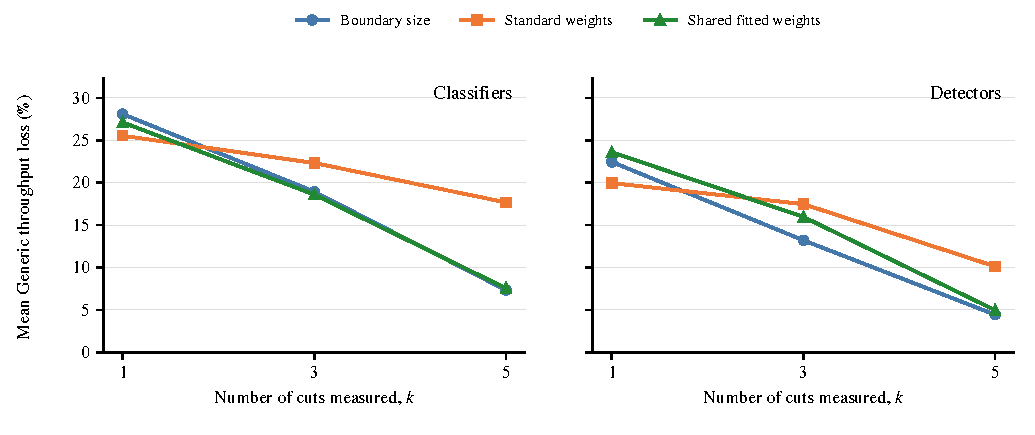
\includegraphics[width=\textwidth]{figures/shortlist_loss.pdf}
\caption{Graph-based selection against measured Generic throughput. Curves show the mean throughput loss after measuring the first $k$ ranked cuts and retaining the fastest, for classifiers and detectors separately. A budget of 1, 3, or 5 means that many cuts are measured, not that many models are held out. Groups with fewer candidates use all available cuts. The shared score is trained on the other models, excluding the test model on all accelerators. One ranking per test model is evaluated at all three budgets. The training objective averages losses at 1, 3, and 5 cuts. Groups contribute equally. Available conditional snapshot: 331 quality-eligible cuts in 21 model--accelerator groups. Measured quality failures (28) and pending quality decisions (0) are excluded; pending decisions keep the quality universe incomplete.}
\label{fig:rq3-shortlist-loss}
\end{figure*}

% shortlist_loss_single_column
\begin{figure}[t]
\centering
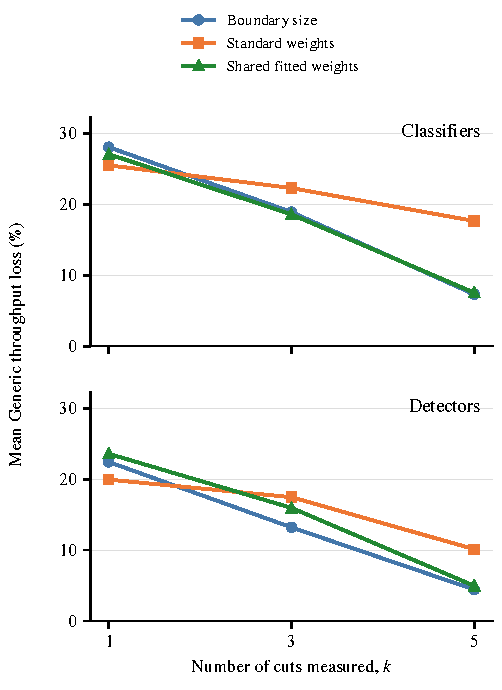
\includegraphics[width=\columnwidth]{figures/shortlist_loss_single_column.pdf}
\caption{Graph-based selection against measured Generic throughput. Curves show the mean throughput loss after measuring the first $k$ ranked cuts and retaining the fastest, for classifiers and detectors separately. A budget of 1, 3, or 5 means that many cuts are measured, not that many models are held out. Groups with fewer candidates use all available cuts. The shared score is trained on the other models, excluding the test model on all accelerators. One ranking per test model is evaluated at all three budgets. The training objective averages losses at 1, 3, and 5 cuts. Groups contribute equally. Available conditional snapshot: 331 quality-eligible cuts in 21 model--accelerator groups. Measured quality failures (28) and pending quality decisions (0) are excluded; pending decisions keep the quality universe incomplete.}
\label{fig:rq3-shortlist-loss-single-column}
\end{figure}

% fit_scopes_k5
\begin{figure*}[t]
\centering
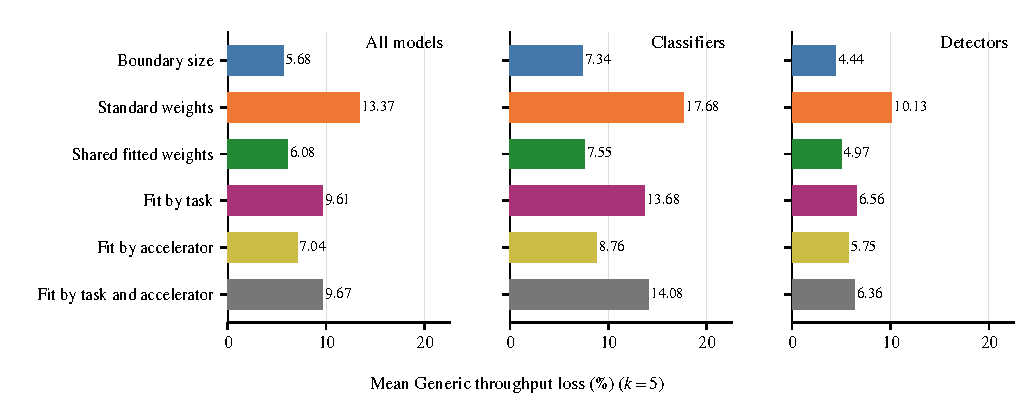
\includegraphics[width=\textwidth]{figures/fit_scopes_k5.pdf}
\caption{Mean Generic throughput loss with a budget of five cuts. Shared weights are compared with separate fits by task, accelerator, or their combination. Every fit holds out the complete test model on all accelerators and is trained on the mean loss at budgets 1, 3, and 5. Values describe the available quality-eligible snapshot, not new Native measurements.}
\label{fig:rq3-fit-scopes-k5}
\end{figure*}
